% Created by tikzDevice version 0.12 on 2019-02-01 11:29:58
% !TEX encoding = UTF-8 Unicode
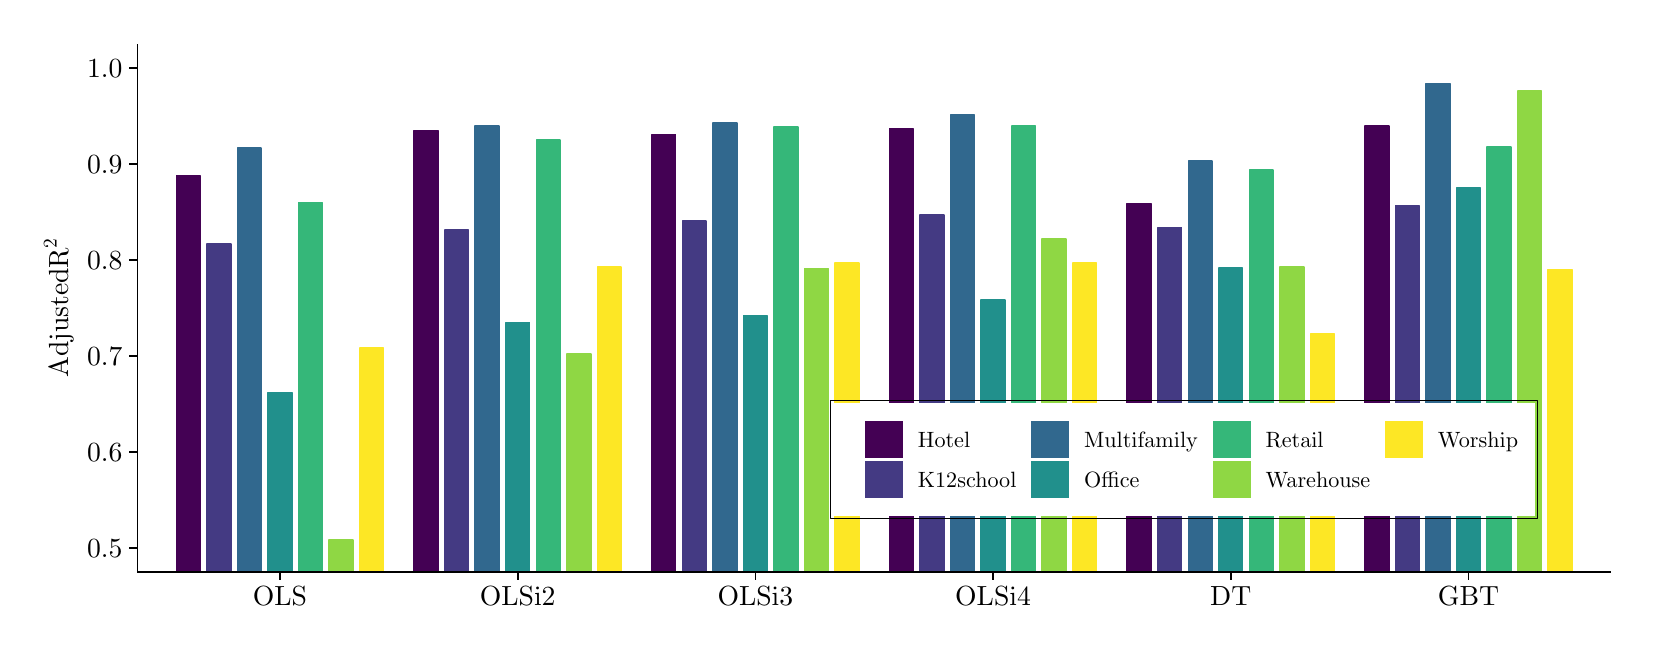
\begin{tikzpicture}[x=1pt,y=1pt]
\definecolor{fillColor}{RGB}{255,255,255}
\path[use as bounding box,fill=fillColor,fill opacity=0.00] (0,0) rectangle (578.16,216.81);
\begin{scope}
\path[clip] (  0.00,  0.00) rectangle (578.16,216.81);
\definecolor{drawColor}{RGB}{255,255,255}
\definecolor{fillColor}{RGB}{255,255,255}

\path[draw=drawColor,line width= 0.6pt,line join=round,line cap=round,fill=fillColor] (  0.00,  0.00) rectangle (578.16,216.81);
\end{scope}
\begin{scope}
\path[clip] ( 39.64, 20.23) rectangle (572.16,210.81);
\definecolor{fillColor}{RGB}{255,255,255}

\path[fill=fillColor] ( 39.64, 20.23) rectangle (572.16,210.81);
\definecolor{drawColor}{RGB}{253,231,37}
\definecolor{fillColor}{RGB}{253,231,37}

\path[draw=drawColor,line width= 0.6pt,line join=round,fill=fillColor] (120.01,-144.36) rectangle (128.60,100.97);
\definecolor{drawColor}{RGB}{143,215,68}
\definecolor{fillColor}{RGB}{143,215,68}

\path[draw=drawColor,line width= 0.6pt,line join=round,fill=fillColor] (108.97,-144.36) rectangle (117.56, 31.67);
\definecolor{drawColor}{RGB}{53,183,121}
\definecolor{fillColor}{RGB}{53,183,121}

\path[draw=drawColor,line width= 0.6pt,line join=round,fill=fillColor] ( 97.92,-144.36) rectangle (106.51,153.64);
\definecolor{drawColor}{RGB}{33,144,140}
\definecolor{fillColor}{RGB}{33,144,140}

\path[draw=drawColor,line width= 0.6pt,line join=round,fill=fillColor] ( 86.88,-144.36) rectangle ( 95.47, 85.03);
\definecolor{drawColor}{RGB}{49,104,142}
\definecolor{fillColor}{RGB}{49,104,142}

\path[draw=drawColor,line width= 0.6pt,line join=round,fill=fillColor] ( 75.84,-144.36) rectangle ( 84.43,173.39);
\definecolor{drawColor}{RGB}{68,58,131}
\definecolor{fillColor}{RGB}{68,58,131}

\path[draw=drawColor,line width= 0.6pt,line join=round,fill=fillColor] ( 64.80,-144.36) rectangle ( 73.38,138.74);
\definecolor{drawColor}{RGB}{68,1,84}
\definecolor{fillColor}{RGB}{68,1,84}

\path[draw=drawColor,line width= 0.6pt,line join=round,fill=fillColor] ( 53.75,-144.36) rectangle ( 62.34,163.34);
\definecolor{drawColor}{RGB}{253,231,37}
\definecolor{fillColor}{RGB}{253,231,37}

\path[draw=drawColor,line width= 0.6pt,line join=round,fill=fillColor] (205.90,-144.36) rectangle (214.49,130.42);
\definecolor{drawColor}{RGB}{143,215,68}
\definecolor{fillColor}{RGB}{143,215,68}

\path[draw=drawColor,line width= 0.6pt,line join=round,fill=fillColor] (194.86,-144.36) rectangle (203.45, 98.89);
\definecolor{drawColor}{RGB}{53,183,121}
\definecolor{fillColor}{RGB}{53,183,121}

\path[draw=drawColor,line width= 0.6pt,line join=round,fill=fillColor] (183.81,-144.36) rectangle (192.40,176.16);
\definecolor{drawColor}{RGB}{33,144,140}
\definecolor{fillColor}{RGB}{33,144,140}

\path[draw=drawColor,line width= 0.6pt,line join=round,fill=fillColor] (172.77,-144.36) rectangle (181.36,110.32);
\definecolor{drawColor}{RGB}{49,104,142}
\definecolor{fillColor}{RGB}{49,104,142}

\path[draw=drawColor,line width= 0.6pt,line join=round,fill=fillColor] (161.73,-144.36) rectangle (170.32,181.36);
\definecolor{drawColor}{RGB}{68,58,131}
\definecolor{fillColor}{RGB}{68,58,131}

\path[draw=drawColor,line width= 0.6pt,line join=round,fill=fillColor] (150.69,-144.36) rectangle (159.27,143.59);
\definecolor{drawColor}{RGB}{68,1,84}
\definecolor{fillColor}{RGB}{68,1,84}

\path[draw=drawColor,line width= 0.6pt,line join=round,fill=fillColor] (139.64,-144.36) rectangle (148.23,179.62);
\definecolor{drawColor}{RGB}{253,231,37}
\definecolor{fillColor}{RGB}{253,231,37}

\path[draw=drawColor,line width= 0.6pt,line join=round,fill=fillColor] (291.79,-144.36) rectangle (300.38,131.81);
\definecolor{drawColor}{RGB}{143,215,68}
\definecolor{fillColor}{RGB}{143,215,68}

\path[draw=drawColor,line width= 0.6pt,line join=round,fill=fillColor] (280.75,-144.36) rectangle (289.34,129.73);
\definecolor{drawColor}{RGB}{53,183,121}
\definecolor{fillColor}{RGB}{53,183,121}

\path[draw=drawColor,line width= 0.6pt,line join=round,fill=fillColor] (269.70,-144.36) rectangle (278.29,181.01);
\definecolor{drawColor}{RGB}{33,144,140}
\definecolor{fillColor}{RGB}{33,144,140}

\path[draw=drawColor,line width= 0.6pt,line join=round,fill=fillColor] (258.66,-144.36) rectangle (267.25,112.75);
\definecolor{drawColor}{RGB}{49,104,142}
\definecolor{fillColor}{RGB}{49,104,142}

\path[draw=drawColor,line width= 0.6pt,line join=round,fill=fillColor] (247.62,-144.36) rectangle (256.21,182.40);
\definecolor{drawColor}{RGB}{68,58,131}
\definecolor{fillColor}{RGB}{68,58,131}

\path[draw=drawColor,line width= 0.6pt,line join=round,fill=fillColor] (236.58,-144.36) rectangle (245.16,147.05);
\definecolor{drawColor}{RGB}{68,1,84}
\definecolor{fillColor}{RGB}{68,1,84}

\path[draw=drawColor,line width= 0.6pt,line join=round,fill=fillColor] (225.53,-144.36) rectangle (234.12,178.24);
\definecolor{drawColor}{RGB}{253,231,37}
\definecolor{fillColor}{RGB}{253,231,37}

\path[draw=drawColor,line width= 0.6pt,line join=round,fill=fillColor] (377.68,-144.36) rectangle (386.27,131.81);
\definecolor{drawColor}{RGB}{143,215,68}
\definecolor{fillColor}{RGB}{143,215,68}

\path[draw=drawColor,line width= 0.6pt,line join=round,fill=fillColor] (366.64,-144.36) rectangle (375.23,140.47);
\definecolor{drawColor}{RGB}{53,183,121}
\definecolor{fillColor}{RGB}{53,183,121}

\path[draw=drawColor,line width= 0.6pt,line join=round,fill=fillColor] (355.59,-144.36) rectangle (364.18,181.36);
\definecolor{drawColor}{RGB}{33,144,140}
\definecolor{fillColor}{RGB}{33,144,140}

\path[draw=drawColor,line width= 0.6pt,line join=round,fill=fillColor] (344.55,-144.36) rectangle (353.14,118.29);
\definecolor{drawColor}{RGB}{49,104,142}
\definecolor{fillColor}{RGB}{49,104,142}

\path[draw=drawColor,line width= 0.6pt,line join=round,fill=fillColor] (333.51,-144.36) rectangle (342.10,185.17);
\definecolor{drawColor}{RGB}{68,58,131}
\definecolor{fillColor}{RGB}{68,58,131}

\path[draw=drawColor,line width= 0.6pt,line join=round,fill=fillColor] (322.47,-144.36) rectangle (331.05,149.13);
\definecolor{drawColor}{RGB}{68,1,84}
\definecolor{fillColor}{RGB}{68,1,84}

\path[draw=drawColor,line width= 0.6pt,line join=round,fill=fillColor] (311.42,-144.36) rectangle (320.01,180.32);
\definecolor{drawColor}{RGB}{253,231,37}
\definecolor{fillColor}{RGB}{253,231,37}

\path[draw=drawColor,line width= 0.6pt,line join=round,fill=fillColor] (463.57,-144.36) rectangle (472.16,106.16);
\definecolor{drawColor}{RGB}{143,215,68}
\definecolor{fillColor}{RGB}{143,215,68}

\path[draw=drawColor,line width= 0.6pt,line join=round,fill=fillColor] (452.53,-144.36) rectangle (461.12,130.42);
\definecolor{drawColor}{RGB}{53,183,121}
\definecolor{fillColor}{RGB}{53,183,121}

\path[draw=drawColor,line width= 0.6pt,line join=round,fill=fillColor] (441.48,-144.36) rectangle (450.07,165.42);
\definecolor{drawColor}{RGB}{33,144,140}
\definecolor{fillColor}{RGB}{33,144,140}

\path[draw=drawColor,line width= 0.6pt,line join=round,fill=fillColor] (430.44,-144.36) rectangle (439.03,130.07);
\definecolor{drawColor}{RGB}{49,104,142}
\definecolor{fillColor}{RGB}{49,104,142}

\path[draw=drawColor,line width= 0.6pt,line join=round,fill=fillColor] (419.40,-144.36) rectangle (427.99,168.54);
\definecolor{drawColor}{RGB}{68,58,131}
\definecolor{fillColor}{RGB}{68,58,131}

\path[draw=drawColor,line width= 0.6pt,line join=round,fill=fillColor] (408.36,-144.36) rectangle (416.94,144.63);
\definecolor{drawColor}{RGB}{68,1,84}
\definecolor{fillColor}{RGB}{68,1,84}

\path[draw=drawColor,line width= 0.6pt,line join=round,fill=fillColor] (397.31,-144.36) rectangle (405.90,153.29);
\definecolor{drawColor}{RGB}{253,231,37}
\definecolor{fillColor}{RGB}{253,231,37}

\path[draw=drawColor,line width= 0.6pt,line join=round,fill=fillColor] (549.46,-144.36) rectangle (558.05,129.38);
\definecolor{drawColor}{RGB}{143,215,68}
\definecolor{fillColor}{RGB}{143,215,68}

\path[draw=drawColor,line width= 0.6pt,line join=round,fill=fillColor] (538.42,-144.36) rectangle (547.01,193.83);
\definecolor{drawColor}{RGB}{53,183,121}
\definecolor{fillColor}{RGB}{53,183,121}

\path[draw=drawColor,line width= 0.6pt,line join=round,fill=fillColor] (527.37,-144.36) rectangle (535.96,173.73);
\definecolor{drawColor}{RGB}{33,144,140}
\definecolor{fillColor}{RGB}{33,144,140}

\path[draw=drawColor,line width= 0.6pt,line join=round,fill=fillColor] (516.33,-144.36) rectangle (524.92,158.83);
\definecolor{drawColor}{RGB}{49,104,142}
\definecolor{fillColor}{RGB}{49,104,142}

\path[draw=drawColor,line width= 0.6pt,line join=round,fill=fillColor] (505.29,-144.36) rectangle (513.88,196.60);
\definecolor{drawColor}{RGB}{68,58,131}
\definecolor{fillColor}{RGB}{68,58,131}

\path[draw=drawColor,line width= 0.6pt,line join=round,fill=fillColor] (494.25,-144.36) rectangle (502.83,152.60);
\definecolor{drawColor}{RGB}{68,1,84}
\definecolor{fillColor}{RGB}{68,1,84}

\path[draw=drawColor,line width= 0.6pt,line join=round,fill=fillColor] (483.20,-144.36) rectangle (491.79,181.36);
\end{scope}
\begin{scope}
\path[clip] (  0.00,  0.00) rectangle (578.16,216.81);
\definecolor{drawColor}{RGB}{0,0,0}

\path[draw=drawColor,line width= 0.6pt,line join=round] ( 39.64, 20.23) --
	( 39.64,210.81);
\end{scope}
\begin{scope}
\path[clip] (  0.00,  0.00) rectangle (578.16,216.81);
\definecolor{drawColor}{RGB}{0,0,0}

\node[text=drawColor,anchor=base east,inner sep=0pt, outer sep=0pt, scale=  1.00] at ( 34.24, 25.45) {0.5};

\node[text=drawColor,anchor=base east,inner sep=0pt, outer sep=0pt, scale=  1.00] at ( 34.24, 60.10) {0.6};

\node[text=drawColor,anchor=base east,inner sep=0pt, outer sep=0pt, scale=  1.00] at ( 34.24, 94.75) {0.7};

\node[text=drawColor,anchor=base east,inner sep=0pt, outer sep=0pt, scale=  1.00] at ( 34.24,129.40) {0.8};

\node[text=drawColor,anchor=base east,inner sep=0pt, outer sep=0pt, scale=  1.00] at ( 34.24,164.05) {0.9};

\node[text=drawColor,anchor=base east,inner sep=0pt, outer sep=0pt, scale=  1.00] at ( 34.24,198.70) {1.0};
\end{scope}
\begin{scope}
\path[clip] (  0.00,  0.00) rectangle (578.16,216.81);
\definecolor{drawColor}{RGB}{0,0,0}

\path[draw=drawColor,line width= 0.6pt,line join=round] ( 36.64, 28.89) --
	( 39.64, 28.89);

\path[draw=drawColor,line width= 0.6pt,line join=round] ( 36.64, 63.54) --
	( 39.64, 63.54);

\path[draw=drawColor,line width= 0.6pt,line join=round] ( 36.64, 98.20) --
	( 39.64, 98.20);

\path[draw=drawColor,line width= 0.6pt,line join=round] ( 36.64,132.85) --
	( 39.64,132.85);

\path[draw=drawColor,line width= 0.6pt,line join=round] ( 36.64,167.50) --
	( 39.64,167.50);

\path[draw=drawColor,line width= 0.6pt,line join=round] ( 36.64,202.15) --
	( 39.64,202.15);
\end{scope}
\begin{scope}
\path[clip] (  0.00,  0.00) rectangle (578.16,216.81);
\definecolor{drawColor}{RGB}{0,0,0}

\path[draw=drawColor,line width= 0.6pt,line join=round] ( 39.64, 20.23) --
	(572.16, 20.23);
\end{scope}
\begin{scope}
\path[clip] (  0.00,  0.00) rectangle (578.16,216.81);
\definecolor{drawColor}{RGB}{0,0,0}

\path[draw=drawColor,line width= 0.6pt,line join=round] ( 91.18, 17.23) --
	( 91.18, 20.23);

\path[draw=drawColor,line width= 0.6pt,line join=round] (177.07, 17.23) --
	(177.07, 20.23);

\path[draw=drawColor,line width= 0.6pt,line join=round] (262.96, 17.23) --
	(262.96, 20.23);

\path[draw=drawColor,line width= 0.6pt,line join=round] (348.85, 17.23) --
	(348.85, 20.23);

\path[draw=drawColor,line width= 0.6pt,line join=round] (434.74, 17.23) --
	(434.74, 20.23);

\path[draw=drawColor,line width= 0.6pt,line join=round] (520.63, 17.23) --
	(520.63, 20.23);
\end{scope}
\begin{scope}
\path[clip] (  0.00,  0.00) rectangle (578.16,216.81);
\definecolor{drawColor}{RGB}{0,0,0}

\node[text=drawColor,anchor=base,inner sep=0pt, outer sep=0pt, scale=  1.00] at ( 91.18,  7.94) {OLS};

\node[text=drawColor,anchor=base,inner sep=0pt, outer sep=0pt, scale=  1.00] at (177.07,  7.94) {OLSi2};

\node[text=drawColor,anchor=base,inner sep=0pt, outer sep=0pt, scale=  1.00] at (262.96,  7.94) {OLSi3};

\node[text=drawColor,anchor=base,inner sep=0pt, outer sep=0pt, scale=  1.00] at (348.85,  7.94) {OLSi4};

\node[text=drawColor,anchor=base,inner sep=0pt, outer sep=0pt, scale=  1.00] at (434.74,  7.94) {DT};

\node[text=drawColor,anchor=base,inner sep=0pt, outer sep=0pt, scale=  1.00] at (520.63,  7.94) {GBT};
\end{scope}
\begin{scope}
\path[clip] (  0.00,  0.00) rectangle (578.16,216.81);
\definecolor{drawColor}{RGB}{0,0,0}

\node[text=drawColor,rotate= 90.00,anchor=base west,inner sep=0pt, outer sep=0pt, scale=  1.00] at ( 14.58, 90.49) {Adjusted };

\node[text=drawColor,rotate= 90.00,anchor=base west,inner sep=0pt, outer sep=0pt, scale=  1.00] at ( 14.58,129.70) {R};

\node[text=drawColor,rotate= 90.00,anchor=base west,inner sep=0pt, outer sep=0pt, scale=  0.70] at ( 10.49,137.06) {2};
\end{scope}
\begin{scope}
\path[clip] (  0.00,  0.00) rectangle (578.16,216.81);
\definecolor{drawColor}{RGB}{0,0,0}

\path[draw=drawColor,line width= 0.4pt,line join=round,line cap=round] (290.24, 39.29) rectangle (545.53, 82.20);
\end{scope}
\begin{scope}
\path[clip] (  0.00,  0.00) rectangle (578.16,216.81);
\definecolor{fillColor}{RGB}{255,255,255}

\path[fill=fillColor] (291.24, 40.29) rectangle (544.53, 81.20);
\end{scope}
\begin{scope}
\path[clip] (  0.00,  0.00) rectangle (578.16,216.81);
\definecolor{drawColor}{RGB}{68,1,84}
\definecolor{fillColor}{RGB}{68,1,84}

\path[draw=drawColor,line width= 0.6pt,line cap=round,fill=fillColor] (302.95, 61.45) rectangle (315.98, 74.49);
\end{scope}
\begin{scope}
\path[clip] (  0.00,  0.00) rectangle (578.16,216.81);
\definecolor{drawColor}{RGB}{68,58,131}
\definecolor{fillColor}{RGB}{68,58,131}

\path[draw=drawColor,line width= 0.6pt,line cap=round,fill=fillColor] (302.95, 47.00) rectangle (315.98, 60.03);
\end{scope}
\begin{scope}
\path[clip] (  0.00,  0.00) rectangle (578.16,216.81);
\definecolor{drawColor}{RGB}{49,104,142}
\definecolor{fillColor}{RGB}{49,104,142}

\path[draw=drawColor,line width= 0.6pt,line cap=round,fill=fillColor] (363.00, 61.45) rectangle (376.03, 74.49);
\end{scope}
\begin{scope}
\path[clip] (  0.00,  0.00) rectangle (578.16,216.81);
\definecolor{drawColor}{RGB}{33,144,140}
\definecolor{fillColor}{RGB}{33,144,140}

\path[draw=drawColor,line width= 0.6pt,line cap=round,fill=fillColor] (363.00, 47.00) rectangle (376.03, 60.03);
\end{scope}
\begin{scope}
\path[clip] (  0.00,  0.00) rectangle (578.16,216.81);
\definecolor{drawColor}{RGB}{53,183,121}
\definecolor{fillColor}{RGB}{53,183,121}

\path[draw=drawColor,line width= 0.6pt,line cap=round,fill=fillColor] (428.55, 61.45) rectangle (441.58, 74.49);
\end{scope}
\begin{scope}
\path[clip] (  0.00,  0.00) rectangle (578.16,216.81);
\definecolor{drawColor}{RGB}{143,215,68}
\definecolor{fillColor}{RGB}{143,215,68}

\path[draw=drawColor,line width= 0.6pt,line cap=round,fill=fillColor] (428.55, 47.00) rectangle (441.58, 60.03);
\end{scope}
\begin{scope}
\path[clip] (  0.00,  0.00) rectangle (578.16,216.81);
\definecolor{drawColor}{RGB}{253,231,37}
\definecolor{fillColor}{RGB}{253,231,37}

\path[draw=drawColor,line width= 0.6pt,line cap=round,fill=fillColor] (490.84, 61.45) rectangle (503.87, 74.49);
\end{scope}
\begin{scope}
\path[clip] (  0.00,  0.00) rectangle (578.16,216.81);
\definecolor{drawColor}{RGB}{0,0,0}

\node[text=drawColor,anchor=base west,inner sep=0pt, outer sep=0pt, scale=  0.80] at (321.70, 65.22) {Hotel};
\end{scope}
\begin{scope}
\path[clip] (  0.00,  0.00) rectangle (578.16,216.81);
\definecolor{drawColor}{RGB}{0,0,0}

\node[text=drawColor,anchor=base west,inner sep=0pt, outer sep=0pt, scale=  0.80] at (321.70, 50.76) {K12school};
\end{scope}
\begin{scope}
\path[clip] (  0.00,  0.00) rectangle (578.16,216.81);
\definecolor{drawColor}{RGB}{0,0,0}

\node[text=drawColor,anchor=base west,inner sep=0pt, outer sep=0pt, scale=  0.80] at (381.74, 65.22) {Multifamily};
\end{scope}
\begin{scope}
\path[clip] (  0.00,  0.00) rectangle (578.16,216.81);
\definecolor{drawColor}{RGB}{0,0,0}

\node[text=drawColor,anchor=base west,inner sep=0pt, outer sep=0pt, scale=  0.80] at (381.74, 50.76) {Office};
\end{scope}
\begin{scope}
\path[clip] (  0.00,  0.00) rectangle (578.16,216.81);
\definecolor{drawColor}{RGB}{0,0,0}

\node[text=drawColor,anchor=base west,inner sep=0pt, outer sep=0pt, scale=  0.80] at (447.30, 65.22) {Retail};
\end{scope}
\begin{scope}
\path[clip] (  0.00,  0.00) rectangle (578.16,216.81);
\definecolor{drawColor}{RGB}{0,0,0}

\node[text=drawColor,anchor=base west,inner sep=0pt, outer sep=0pt, scale=  0.80] at (447.30, 50.76) {Warehouse};
\end{scope}
\begin{scope}
\path[clip] (  0.00,  0.00) rectangle (578.16,216.81);
\definecolor{drawColor}{RGB}{0,0,0}

\node[text=drawColor,anchor=base west,inner sep=0pt, outer sep=0pt, scale=  0.80] at (509.59, 65.22) {Worship};
\end{scope}
\end{tikzpicture}
